\documentclass[12pt,a4paper]{article}
\usepackage[utf8]{inputenc}
\usepackage{amsmath}
\usepackage{amsfonts}
\usepackage{amssymb}
\usepackage{float}
\usepackage{pgfplots}

\begin{document}
\section*{Testing of SPHINCS, RSA, and ECDSA}
In this section we will be looking at the performance of SPHINCS, RSA, and ECDSA. These three cryptosystems each sign and verify messages in different ways. Below goes into a quick overview on how each system works. Below is a summary of each the cryptosystems we will be looking at. In the next section we will look at how these three cryptosystems match up against each other.

\subsection*{SPHINCS}
SPHINCS makes use of multiple trees to obtain a few time signature (FTS) scheme. This is done using a mixture of Winternitz one time signatures + (WOTS+) and HORS with trees (HORST). The idea of SPHINCS uses a hyper-tree which is borrowed from an idea by Goldreich, which turns a stateful scheme into a stateless scheme. WOTS+ eventually feeds into multiple HORST in the end, which allows for extending signatures to be multi-use instead of single use. SPHINCS has three steps: Key generation, signature generation and signature verification.

\subsection*{RSA}
RSA is used for signing messages by using public-key cryptography. It is an asymmetric cryptosystem that is based on the difficulty of factoring two large prime numbers. With RSA there are four steps we go through: key generation, key distribution, encryption and decryption.

\subsection*{ECDSA}
ECDSA uses elliptic-curve cryptography to obtain the needed parameters. Key generation in ECDSA requires less bits compared to DSA to obtain the same amount of security. The signature size requires the same amount of bit in both ECDSA and DSA to obtain the same amount of security. ECDSA contains three steps: Key generation, signature generation, and signature verification.

\section*{Benchmarks for SPHINCS, RSA, and ECDSA}
Benchmarking is done on Arch Linux (4.4.1-2-ARCH), processor: Intel Quad-Core i7-4710HQ 2.50GHz, 8 gigabytes RAM). The testing for SPHINCS is done using a python implementation that is not designed for optimization. This implementation was meant to learn and understand how individual pieces of SPHINCS work [1]. There are optimized versions of SPHINCS available, but compiling the from these implementations are very complex. The testing for RSA and ECDSA is done using MIRACL crypto library, which is an optimized library for performance [2].

The benchmarking is ran using different files sizes, ranging from 10 Kb up to 100 Kb with file sizes being increased in 10 Kb increments. Below you will find two different tests for each cryptosystem, signing and verification.

\begin{table} [H]
\centering
\caption{Performance of message signing}
\begin{tabular}{|c|c|c|c|}
\hline 
 & SPHINCS & RSA & ECDSA \\ 
\hline 
10 Kb & 1m 43.597sec & 0.005320ms & 0.000299ms \\ 
\hline 
20 Kb & 1m 42.665sec & 0.009426ms & 0.000480ms \\ 
\hline 
30 Kb & 1m 42.878sec & 0.013967ms & 0.000574ms \\ 
\hline 
40 Kb & 1m 43.089sec & 0.019238ms & 0.000687ms \\ 
\hline 
50 Kb & 1m 42.976sec & 0.023722ms & 0.000911ms \\ 
\hline 
60 Kb & 1m 43.105sec & 0.029159ms & 0.000921ms \\ 
\hline 
70 Kb & 1m 43.738sec & 0.032512ms & 0.001048ms \\ 
\hline 
80 Kb & 1m 44.051sec & 0.037693ms & 0.001293ms \\ 
\hline 
90 Kb & 1m 43.296sec & 0.042439ms & 0.002060ms \\ 
\hline 
100 Kb & 1m 43.495sec & 0.047571ms & 0.001676ms \\ 
\hline 
\end{tabular} 
\end{table}

\begin{table} [H]
\centering
\caption{Performance of message verification}
\begin{tabular}{|c|c|c|c|}
\hline 
 & SPHINCS & RSA & ECDSA \\ 
\hline 
10 Kb & 1.250sec & 0.000097ms & 0.001306ms \\ 
\hline 
20 Kb & 1.232sec & 0.000098ms & 0.001342ms \\ 
\hline 
30 Kb & 1.3sec & 0.000090ms & 0.001531ms \\ 
\hline 
40 Kb & 1.288sec & 0.000111ms & 0.001573ms \\ 
\hline 
50 Kb & 1.318sec & 0.000105ms & 0.001759ms \\ 
\hline 
60 Kb & 1.292sec & 0.000111ms & 0.001859ms \\ 
\hline 
70 Kb & 1.343sec & 0.000099ms & 0.002030ms \\ 
\hline 
80 Kb & 1.394sec & 0.000102ms & 0.002429ms \\ 
\hline 
90 Kb & 1.383sec & 0.000093ms & 0.002274ms \\ 
\hline 
100 Kb & 1.407sec & 0.000113ms & 0.002447ms \\ 
\hline 
\end{tabular} 
\end{table}

Below we will see the data put into another form which might be easier to comprehend the overall performance of each cryptosystem.

\begin{center}
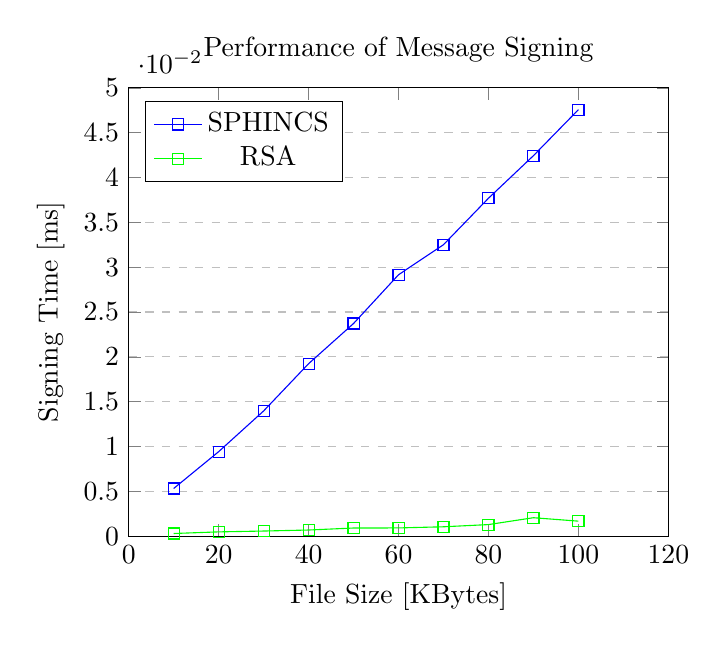
\begin{tikzpicture}
\begin{axis}[
    title={Performance of Message Signing},
    xlabel={File Size [KBytes]},
    ylabel={Signing Time [ms]},
    xmin=0, xmax=120,
    ymin=0, ymax=0.050000,
    xtick={0,20,40,60,80,100,120},
    ytick={0, 0.005 ,0.010 ,0.015 ,0.020, 0.025, 0.030, 0.035, 0.040, 0.045, 0.050},
    legend pos=north west,
    ymajorgrids=true,
    grid style=dashed,
]
 
\addplot[
    color=blue,
    mark=square,
    ]
    coordinates {(10,0.005320)(20,0.009426)(30,0.013967)(40,0.019238)(50,0.023722)(60,0.029159)(70,0.032512)(80,0.037693)(90,0.042439)(100,0.047571)
    };
    
\addplot[
    color=green,
    mark=square,
    ]
    coordinates {(10,0.000299)(20,0.000480)(30,0.000574)(40,0.000687)(50,0.000911)(60,0.000921)(70,0.001048)(80,0.001293)(90,0.002060)(100,0.001676)
    };
    
\legend{SPHINCS, RSA, ECDSA}
 
\end{axis}
\end{tikzpicture}
\end{center}

\begin{center}
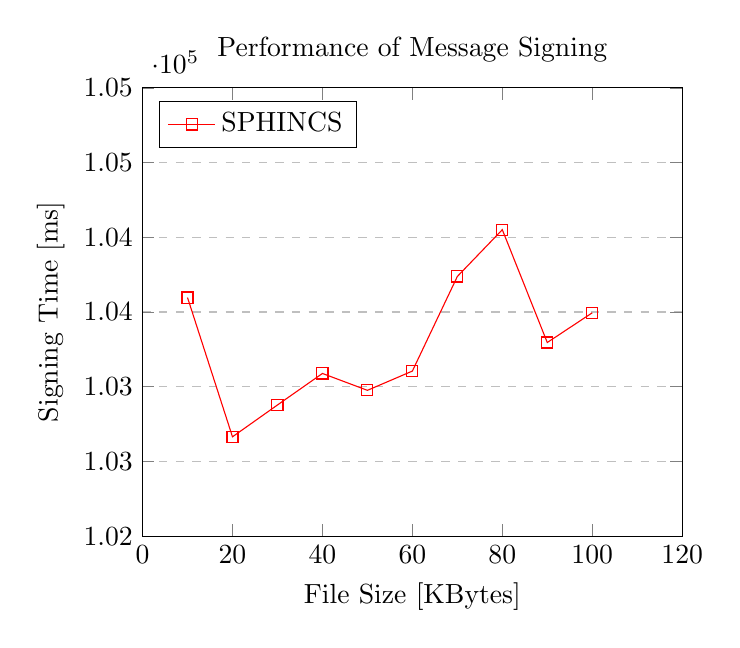
\begin{tikzpicture}
\begin{axis}[
    title={Performance of Message Signing},
    xlabel={File Size [KBytes]},
    ylabel={Signing Time [ms]},
    xmin=0, xmax=120,
    ymin=102000, ymax=105000,
    xtick={0,20,40,60,80,100,120},
    ytick={0,102000,102500,103000,103500,104000,104500,105000},
    legend pos=north west,
    ymajorgrids=true,
    grid style=dashed,
]
 
\addplot[
    color=red,
    mark=square,
    ]
    coordinates {(10,103597)(20,102665)(30,102878)(40,103089)(50,102976)(60,103105)(70,103738)(80,104051)(90,103296)(100,103495)
    };

\legend{SPHINCS}
 
\end{axis}
\end{tikzpicture}
\end{center}

\begin{center}
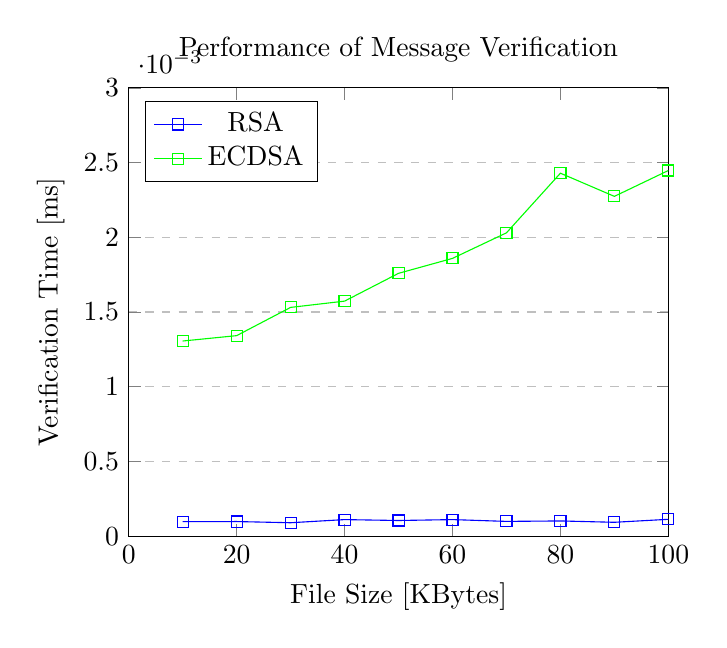
\begin{tikzpicture}
\begin{axis}[
    title={Performance of Message Verification},
    xlabel={File Size [KBytes]},
    ylabel={Verification Time [ms]},
    xmin=0, xmax=100,
    ymin=0, ymax=0.003000,
    xtick={0,20,40,60,80,100},
    ytick={0, 0.0005 ,0.0010 ,0.0015 ,0.0020, 0.0025, 0.0030},
    legend pos=north west,
    ymajorgrids=true,
    grid style=dashed,
]
 
\addplot[
    color=blue,
    mark=square,
    ]
    coordinates {(10,0.000097)(20,0.000098)(30,0.000090)(40,0.000111)(50,0.000105)(60,0.000111)(70,0.000099)(80,0.000102)(90,0.000093)(100,0.000113)
    };
    
\addplot[
    color=green,
    mark=square,
    ]
    coordinates {(10,0.001306)(20,0.001342)(30,0.001531)(40,0.001573)(50,0.001759)(60,0.001859)(70,0.002030)(80,0.002429)(90,0.002274)(100,0.002447)
    };
    
\legend{RSA, ECDSA}
 
\end{axis}
\end{tikzpicture}
\end{center}

\begin{center}
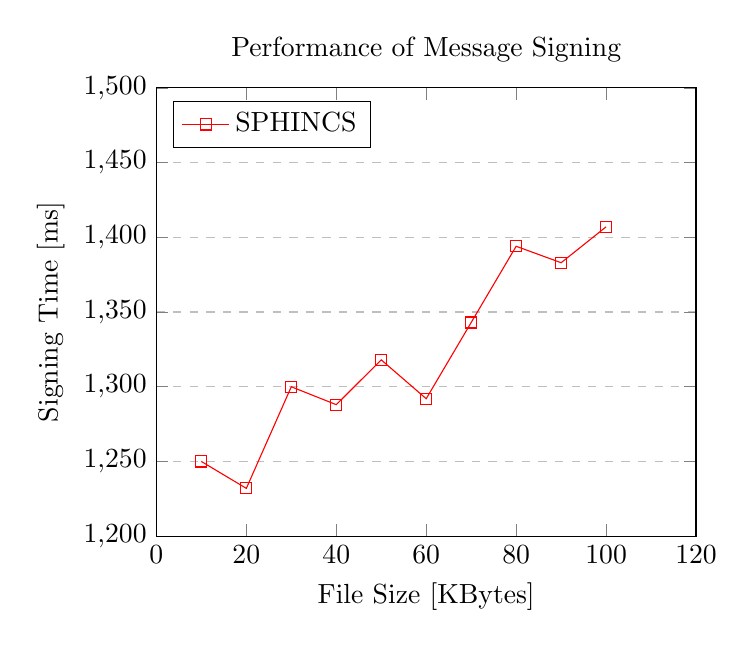
\begin{tikzpicture}
\begin{axis}[
    title={Performance of Message Signing},
    xlabel={File Size [KBytes]},
    ylabel={Signing Time [ms]},
    xmin=0, xmax=120,
    ymin=1200, ymax=1500,
    xtick={0,20,40,60,80,100,120},
    ytick={0,1200,1250,1300,1350,1400,1450,1500},
    legend pos=north west,
    ymajorgrids=true,
    grid style=dashed,
]
 
\addplot[
    color=red,
    mark=square,
    ]
    coordinates {(10,1250)(20,1232)(30,1300)(40,1288)(50,1318)(60,1292)(70,1343)(80,1394)(90,1383)(100,1407)
    };

\legend{SPHINCS}
 
\end{axis}
\end{tikzpicture}
\end{center}

\textbf{NOTE:} Due to SPHINCS performance, it was placed into its own graphs. If it were included in the same graphs with RSA and ECDSA, then they would not be visible.

\section*{Conclusion}
I must stress, as stated in the previous section (Benchmarks), the SPHINCS implementation that was used for this was not optimized at all. The reason for the use of this implementation of SPHINCS was due to ease of use. There are other optimized implementations available, but the complexity to use them is high.

With that being said, as you can see from the graphs above there are trade-offs with using any of these cryptosystems. As file sizes increase the time it takes to sign and verify messages will also increase. 

Based on the implementations used for this benchmark, I would suggest using ECDSA for signatures. ECDSA performs faster than SPHINCS and RSA in terms of signing messages. As you can see though, RSA does verify messages faster than ECDSA, but if you look at the overall performance ECDSA is faster.

\section*{Works Cited}
1) https://github.com/joostrijneveld/SPHINCS-py \\
2) https://github.com/CertiVox/MIRACL

\end{document}